\documentclass{article}

%\usepackage{corl_2023} % Use this for the initial submission.
\usepackage[final]{corl_2023} % Uncomment for the camera-ready ``final'' version.
%\usepackage[preprint]{corl_2023} % Uncomment for pre-prints (e.g., arxiv); This is like ``final'', but will remove the CORL footnote.

\usepackage{graphicx}
\usepackage{amssymb}
\usepackage{amsmath}
\usepackage{listings}
\usepackage{subcaption}
\usepackage{latexsym}
\usepackage{amsthm}
\usepackage{natbib}
\usepackage{listings}
\usepackage{hyperref} 

\title{Exercise 3 - Robot Learning Course}

% The \author macro works with any number of authors. There are two
% commands used to separate the names and addresses of multiple
% authors: \And and \AND.
%
% Using \And between authors leaves it to LaTeX to determine where to
% break the lines. Using \AND forces a line break at that point. So,
% if LaTeX puts 3 of 4 authors names on the first line, and the last
% on the second line, try using \AND instead of \And before the third
% author name.

% NOTE: authors will be visible only in the camera-ready and preprint versions (i.e., when using the option 'final' or 'preprint'). 
% 	For the initial submission the authors will be anonymized.

\author{
  Andrea Ongaro\\
	Computer Engineering\\
	Politecnico di Torino, Italy\\
	\texttt{s329706@studenti.polito.it} \\
  %% examples of more authors
  %% \And
  %% Coauthor \\
  %% Affiliation \\
  %% Address \\
  %% \texttt{email} \\
  %% \AND
  %% Coauthor \\
  %% Affiliation \\
  %% Address \\
  %% \texttt{email} \\
  %% \And
  %% Coauthor \\
  %% Affiliation \\
  %% Address \\
  %% \texttt{email} \\
  %% \And
  %% Coauthor \\
  %% Affiliation \\
  %% Address \\
  %% \texttt{email} \\
}


\begin{document}
\maketitle

%===============================================================================

\begin{abstract}
This article is the third in a series of three reports for the Reinforcement Learning laboratory course at Politecnico di Torino. This report is about policy gradient reinforcement learning algorithms within the OpenAI Gym environment, focusing on the CartPole problem. This process started implementing the naïve REINFORCE algorithm and then exploring more advanced Actor Critic methods like
Proximal Policy Optimization (PPO) and Soft Actor Critic (SAC), also leveraging on the use of well-known
libraries such as Stable-Baselines3.

\end{abstract}

% Two or three meaningful keywords should be added here
\keywords{Reinforcement Learning, Robots, AI} 

%===============================================================================

\section{Introduction}
\subsection{The system - CartPole-v0}
CartPole-v0 system from OpenAI is part of the classic control environment. The starting code it's been provided by \href{https://www.polito.it/personale?p=andrea.protopapa}{Andrea Protopapa} in the course of Reinforcement Learning. Information about this system is sourced from the official documentation \cite{Cart_pole} and its GitHub repository. Below is the definition provided by the authors for CartPole-v0\\ \\
\textit{This environment corresponds to the version of the cart-pole problem described by Barto, Sutton, and Anderson in “Neuronlike Adaptive Elements That Can Solve Difficult Learning Control Problem”. A pole is attached by an un-actuated joint to a cart, which moves along a frictionless track. The pendulum is placed upright on the cart and the goal is to balance the pole by applying forces in the left and right direction on the cart.\citep{Cart_pole}}

For the following procedures, use a modified version of the CartPole environment implemented in cp\_cont.py the standard CartPole uses discrete actions (applying force of either -10 or 10), while in this version it takes actions in the form of a single real number, which represents an arbitrary
force value.
\begin{figure}[h]
	\centering
	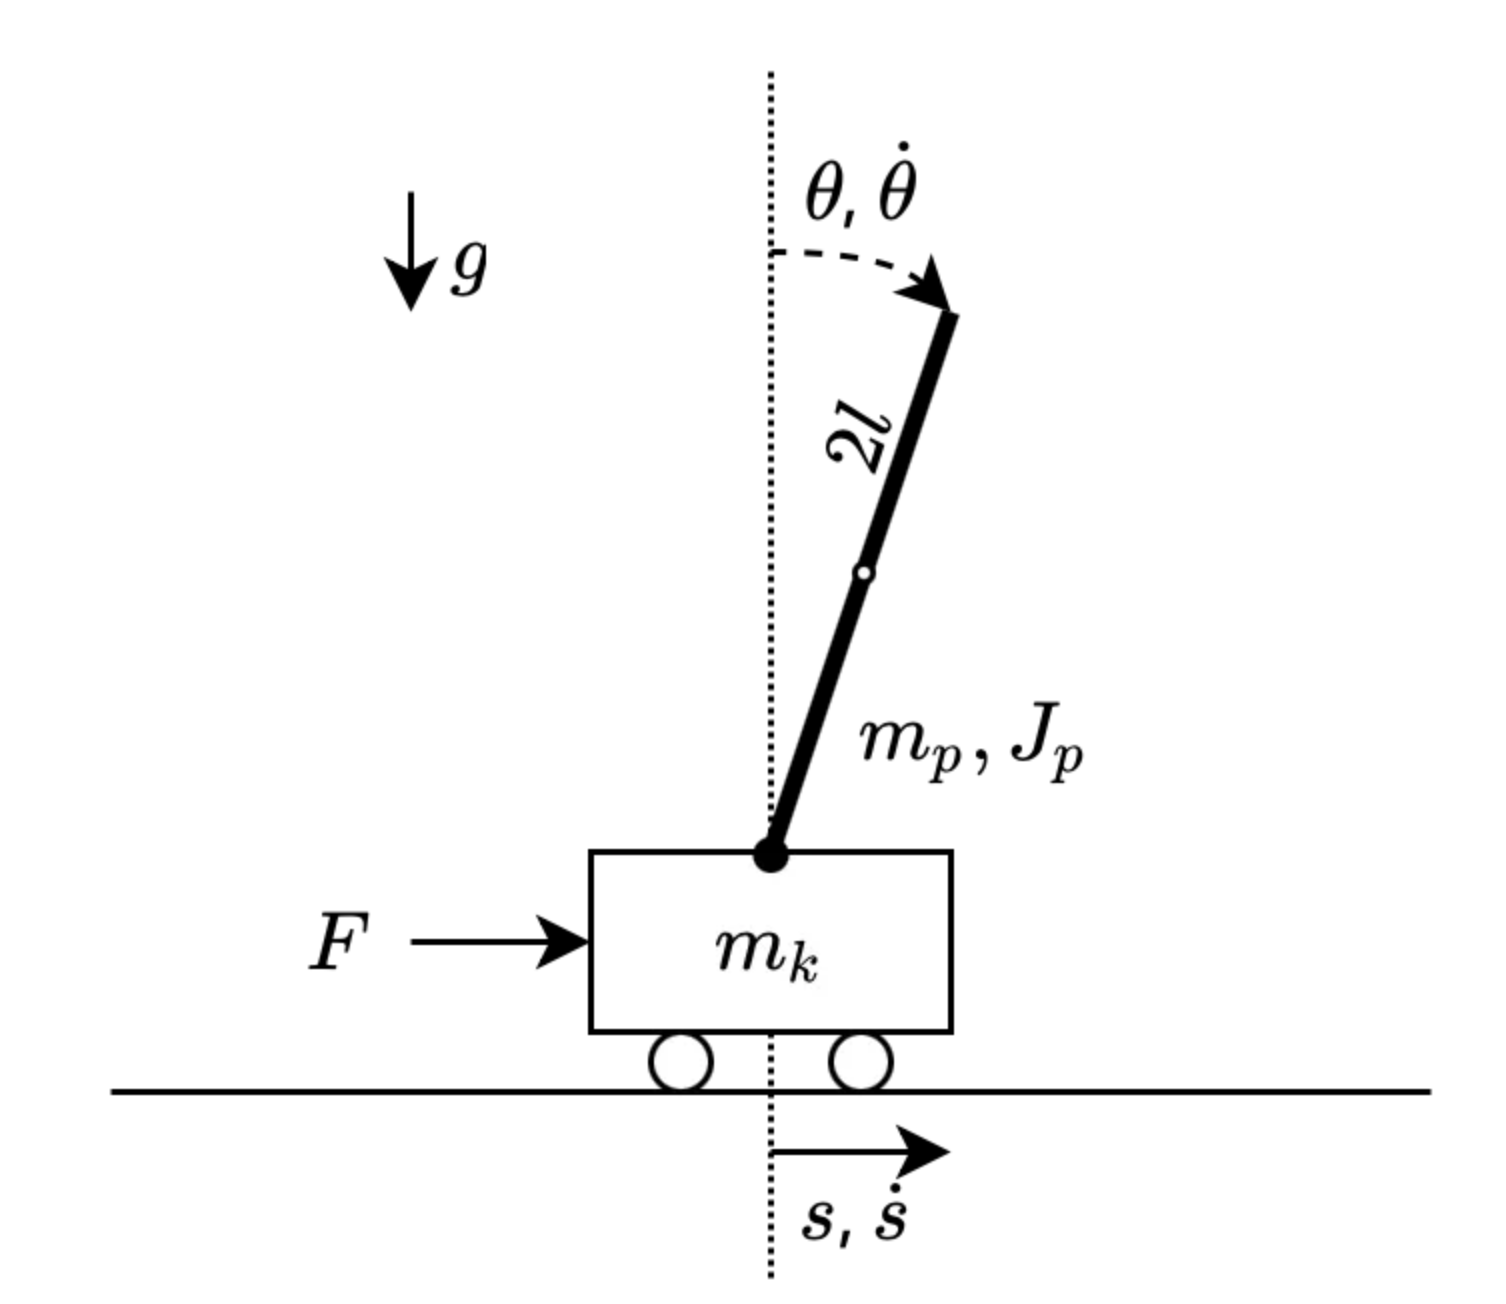
\includegraphics[width=0.5\linewidth]{../data/images/cart.png}
	\caption{Graphical explation about the whole system}
	\label{fig:plot1}
\end{figure}

\newpage

The observation is a four element vector: 
\begin{figure}[h]
	\centering
	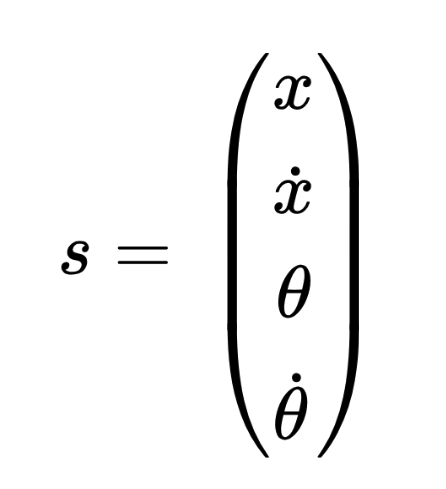
\includegraphics[width=0.2\linewidth]{../data/images/vector.png}
	\caption{Observation vector}
	\label{fig:plot2}
\end{figure}

where 
\begin{itemize}
	\item $x$: the position of the cart
	\item $\dot{x}$: the velocity, 
	\item $\theta$:  the angle of the pole
	\item $\dot{\theta}$: the angular velocity of the pole., 	
\end{itemize}

\section{Policy gradient}

\subsection{REINFORCE algorithm}
REINFORCE is a policy optimization algorithm that directly adjusts the parameters of a stochastic policy to maximize expected cumulative rewards and it operates through gradient ascent as optimization algorithm, iteratively searching for optimal parameters that maximize the objective function. [PROF]

The REINFORCE algorithm can be applied to a wide range of problems, including control tasks, game playing, and robotics. However, it has some limitations, such as high variance in the gradient estimates and slow convergence. To address these issues, various extensions and improvements have been proposed, such as using baseline functions to reduce variance, incorporating advantage estimates, and employing trust region methods.[https://advancedoracademy.medium.com/an-introduction-to-the-reinforce-5470a376b3ab]


\section{Actor Critic}

\subsection{Proximal Policy Optimization (POC)}

\subsection{Soft Actor Critic (SAC)}


\subsection{Stable-Baselines3}
Stable-Baselines 3 is a state-of-the-art RL library offering efficient and stable implementations of various
algorithms. Specifically, it provides robust implementations for PPO and SAC, making it an ideal choice for
experimentation due to its ease of use and reliability. [PROF]

provides open-source implementations of deep reinforcement learning
(RL) algorithms in Python. 

\section{Policy gradient with and without baseline}

Use constant variance for the output action distribution throughout the training.
Implement the following algorithms:
(a) basic REINFORCE without baseline,

\begin{figure}[h]
	\centering
	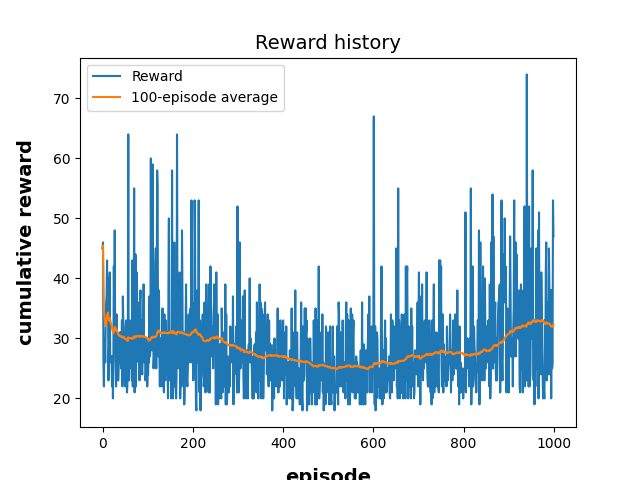
\includegraphics[width=0.5\linewidth]{../data/plot/reward_history_ContinuousCartPole-v0_0_basic.png}
	\caption{Reward history - Basic REINFORCE no baseline}
	\label{fig:plot3}
\end{figure}


(b) REINFORCE with a constant baseline ,

\begin{figure}[h]
	\centering
	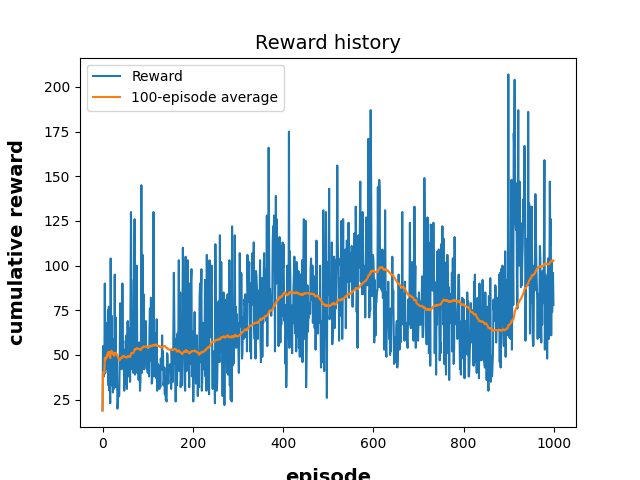
\includegraphics[width=0.5\linewidth]{../data/plot/reward_history_ContinuousCartPole-v0_0_constant_baseline.png}
	\caption{Reward history - Basic REINFORCE with b = 20}
	\label{fig:plot4}
\end{figure}
(c) REINFORCE with discounted rewards normalized to zero mean and unit variance,

A normalized baseline falls under the category of state-independent baselines but with an added transformation for stability. It normalizes the rewards (or returns) by centering them around their mean and scaling them by their standard deviation:

$\text{Normalized Rewards} = \frac{R - \text{mean}(R)}{\text{std}(R) + \epsilon}$

where  $\epsilon$  is a small constant to avoid division by zero.

This type of baseline doesn’t directly depend on the state, but it helps stabilize training by reducing the range and variance of the rewards, which is especially useful when raw rewards vary significantly.

\begin{figure}[h]
	\centering
	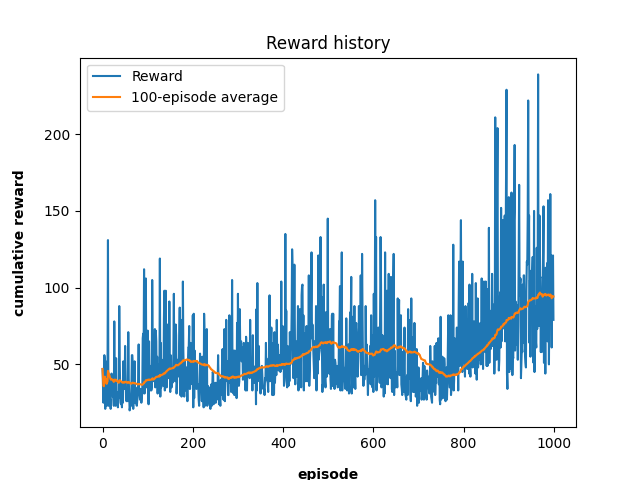
\includegraphics[width=0.5\linewidth]{../data/plot/reward_history_ContinuousCartPole-v0_0_normalized.png}
	\caption{Reward history - Basic REINFORCE with discounted rewards normalized to zero mean and unit variance,}
	\label{fig:plot5}
\end{figure}

\subsection{Baseline value}
\subsection{What is?}
A baseline is a value subtracted from the returns (or rewards) before calculating the gradient of the policy. Its primary purpose is to reduce the variance of gradient estimates, which can make learning more stable and efficient. Importantly, the baseline does not introduce any bias into the gradient computation.[CHATGPT]

Policy gradient methods update the policy parameters based on the estimated advantage of actions:

$\nabla J(\theta) \propto \mathbb{E}[\nabla \log \pi(a|s; \theta) \cdot A(s, a)]$

where  A(s, a)  is the advantage function, which measures how much better an action is compared to some baseline.

Subtracting a baseline  b  from the rewards or returns does not bias the gradient because:

$\mathbb{E}[\nabla \log \pi(a|s; \theta) \cdot b] = 0$

This is because the expectation of the gradient with respect to the policy’s probability distribution over actions sums to zero.\\

Types of Baselines
1.	Constant Baseline:
•	A fixed scalar value (e.g., 0 or the average reward across episodes).
•	Simple to implement but may not capture the variability of rewards in different states.

State-Dependent Baseline:
•	A baseline that depends on the state, such as the value function  V(s) , which estimates the expected return from a state:

$A(s, a) = R\_t - V(s)$

•	Used in Actor-Critic methods, where the critic network estimates  V(s) .

Learned Baseline:
•	A separate neural network trained to approximate the baseline (e.g.,  V(s) ).
•	Dynamically adapts to the agent’s performance.

If  b  is a good approximation of the expected return  $\mathbb{E}[G_t]$ , the variance of  $G_t - b$  is much smaller than  $G_t $

\subsection{Why is important}
A good baseline value is typically chosen based on the following considerations:
Mean of Rewards:
•	The baseline should approximate the average reward over episodes or across states. This reduces variance without introducing bias.
•	Empirical Tuning:
•	Start with simple values (e.g., 0 or the mean reward for a few episodes) and adjust based on training stability.
•	Learned Baseline:
•	Use a separate network to estimate the value function (V(s)) for a state, as in Actor-Critic methods. This allows the baseline to adapt dynamically.

\subsection{Training}
Variance Reduction:
•	A baseline reduces the variance of gradient estimates by subtracting a constant or state-dependent value from rewards. This makes learning more stable and efficient.
•	No Bias Introduction:
•	Subtracting the baseline does not bias the gradient estimation because it does not depend on the actions taken.
•	Impact of Poor Baseline:
•	If the baseline is poorly chosen (e.g., far from the expected reward), it may not reduce variance effectively and could slow down training.


\subsection{Real-world control problems}

\subsection{Risks with Unbounded Continuous Action Spaces and Reward Function}
In a physical system:
•	High Risk of Instability: With unbounded actions, the policy may propose extreme actions, leading to system instability or damage.
•	Reward Gradient Issue: A survival-based reward like +1 offers no penalty for extreme actions unless explicitly constrained. This can mislead the agent into learning aggressive policies that maximize survival without safety considerations.

Question 2.1 What could go wrong when a model with an unbounded continuous action space and a
reward function like the one used here (+1 for survival) were to be used with a physical system?
Question 2.2 How could the problems appearing in Question 2.1 be mitigated without putting a hard limit
on the actions? Explain your answer.

\subsection{Discrete action spaces}
policy gradient methods can be used with discrete action spaces. Here’s why:
•	Action Selection:
•	Instead of sampling from a continuous distribution (e.g., Normal), the policy outputs a probability distribution over discrete actions (e.g., Categorical distribution).
•	Log-Probability:
•	The log-probability of the selected action can still be computed, enabling the gradient update.


Potential Issues with Discrete Action Spaces
1.	Sampling:
•	Actions are sampled from a Categorical distribution. This introduces randomness but is straightforward to implement.
2.	Gradient Estimation:
•	The gradients are computed from the log-probabilities, which are well-defined for discrete actions.
3.	Exploration:
•	Ensuring sufficient exploration is more challenging in discrete spaces but can be addressed with techniques like entropy regularization.

\section{Actor-Critic Methods}

\subsection{Results}
Compare Terms of reward and time consumption.
highlighting any notable differences in terms of learning stability and convergence speed
Additionally, compare the results with the REINFORCE 

\subsection{Hyperparameter modification}
adjust any hyperparameter such as learning rate or others as presented in the documentation if
needed.
%===============================================================================

%===============================================================================

%===============================================================================

% no \bibliographystyle is required, since the corl style is automatically used.
\bibliography{example}  % .bib

\end{document}
